\graphicspath{{main/evaluation/graphics/}}

\chapter{Evaluation}

% This section evaluates the software, hardware or other artefact you have developed.  You should compare it with the original specification and see how well it satisfies the requirements.  You may wish to refer back to your aims and objectives at this point.  You should report the results of user testing and a summary of feedback if that has been collected.

% Evaluation should be rigorous and objective.  Avoid opinion and unsubstantiated statements.
% If you have done experiments, then the results of these should be reported and discussed here.
% If you have involved people in doing user evaluations, that information should be include here.

% Students will be able to review, reflect and document consequences of personal decisions that impact upon their capacity to study effectively and on their general well-being. Review, reflect, plan and maintain a diverse professional portfolio of experience that fosters life-long learning.

\section{Test Harness}

\begin{figure}[ht]
    \centering
    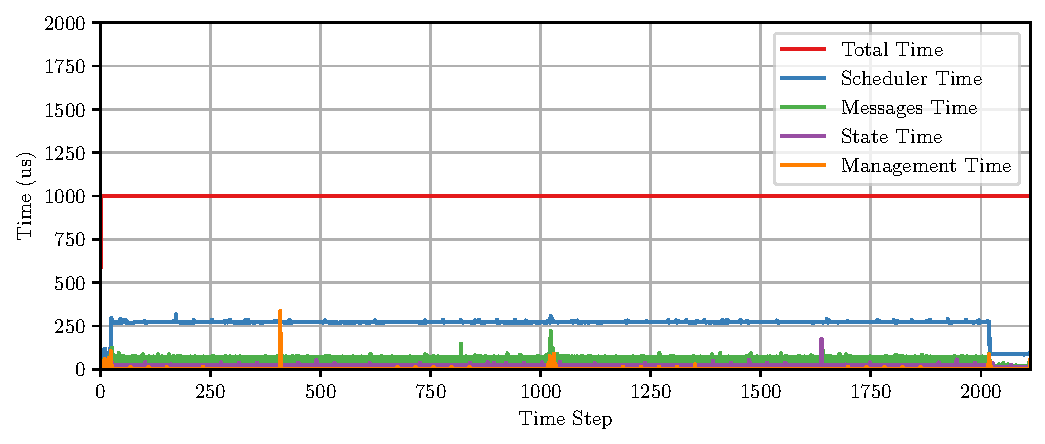
\includegraphics[width=\textwidth]{elafry-harness-times.pdf}
    \caption[Test harness execution times]
    {Test harness execution times}
    \label{fig:testHarnessExecutionTimes}
\end{figure}

\begin{figure}[ht]
    \centering
    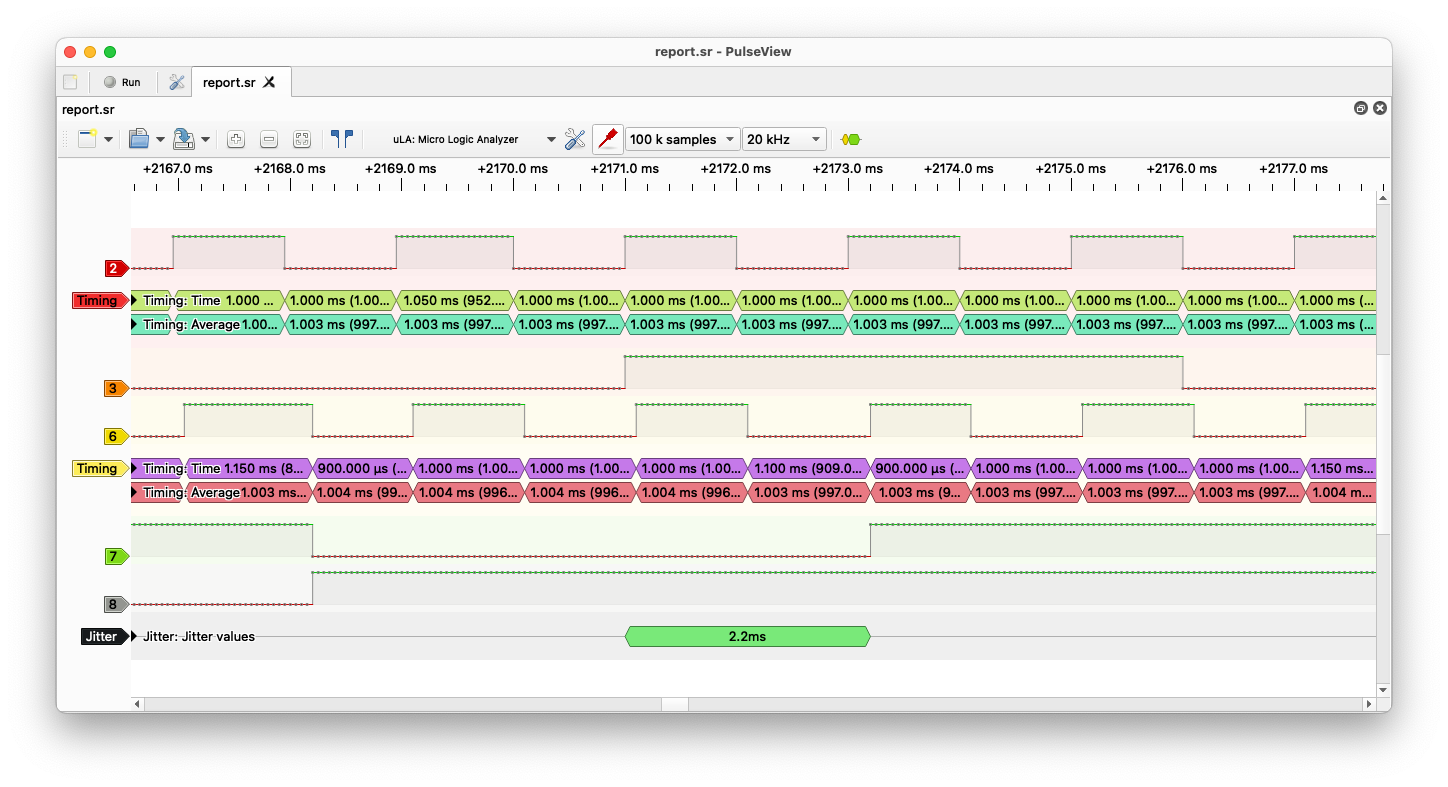
\includegraphics[width=\textwidth]{logic-zoom1}
    \caption[Test harness logic analyser]
    {Test harness logic analyser}
    \label{fig:testHarnessLogicAnalyser}
\end{figure}

\begin{figure}[ht]
    \centering
    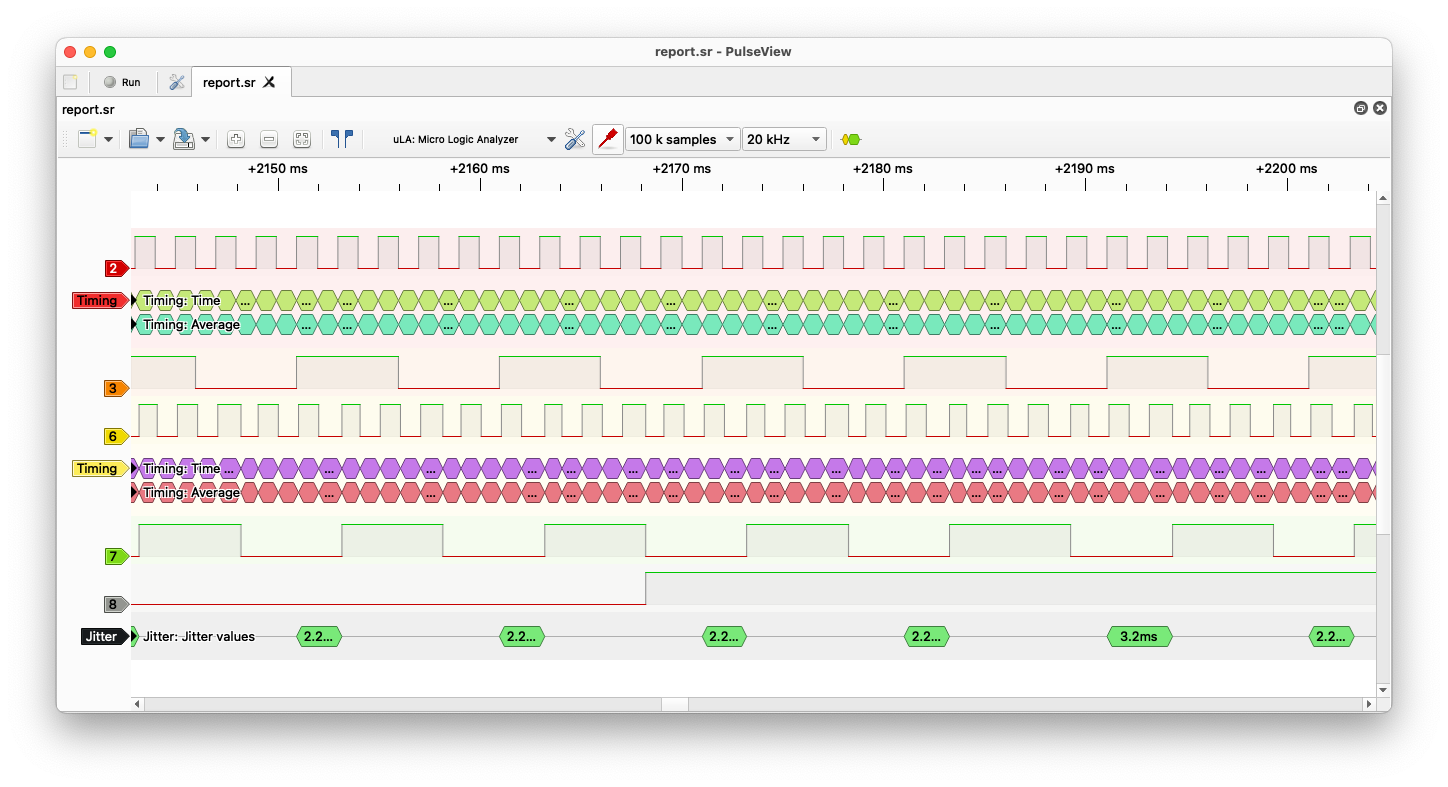
\includegraphics[width=\textwidth]{logic-zoom3}
    \caption[Test harness logic analyser (view)]
    {Test harness logic analyser (view)}
    \label{fig:testHarnessLogicAnalyserView}
\end{figure}

\clearpage

\section{Plant Experiment}

\begin{figure}[ht]
    \centering
    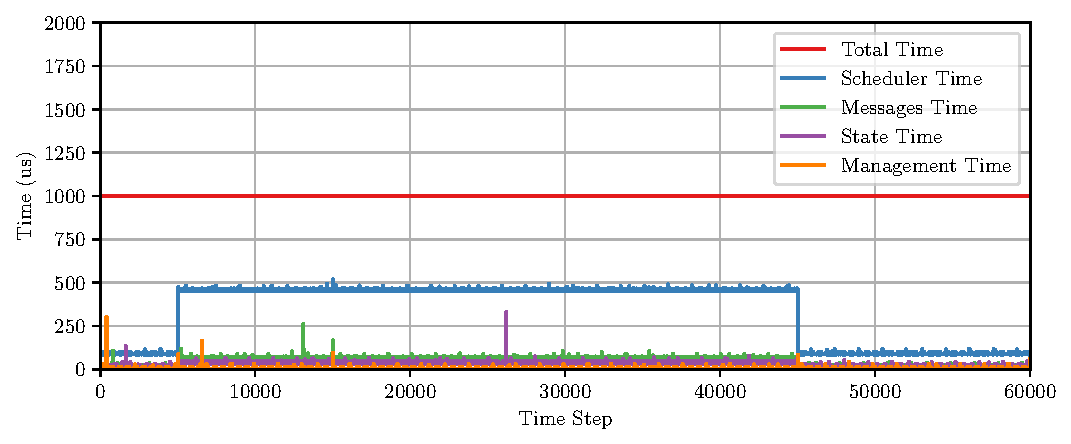
\includegraphics[width=\textwidth]{elafry-plant-times.pdf}
    \caption[Test plant execution times]
    {Test plant execution times}
    \label{fig:testPlantExecutionTimes}
\end{figure}

\begin{figure}[ht]
    \centering
    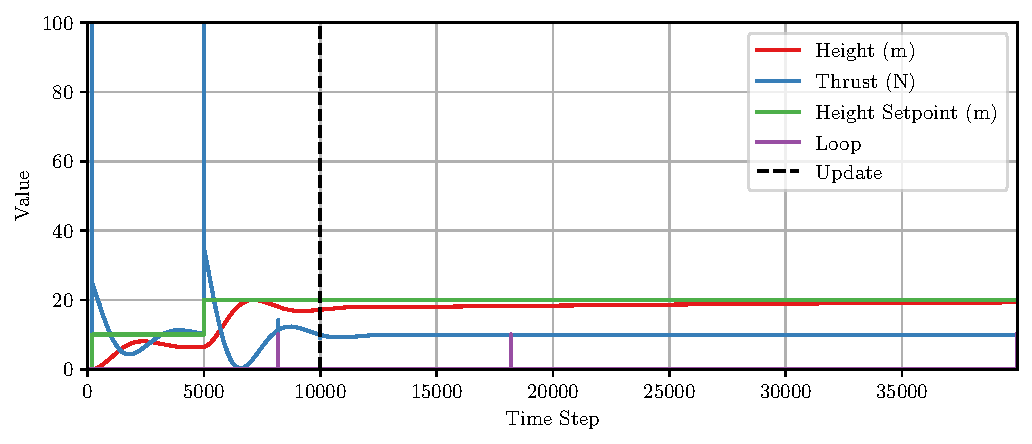
\includegraphics[width=\textwidth]{elafry-plant-data.pdf}
    \caption[Test plant control view]
    {Test plant control view}
    \label{fig:testPlantControlView}
\end{figure}

\begin{figure}[ht]
    \centering
    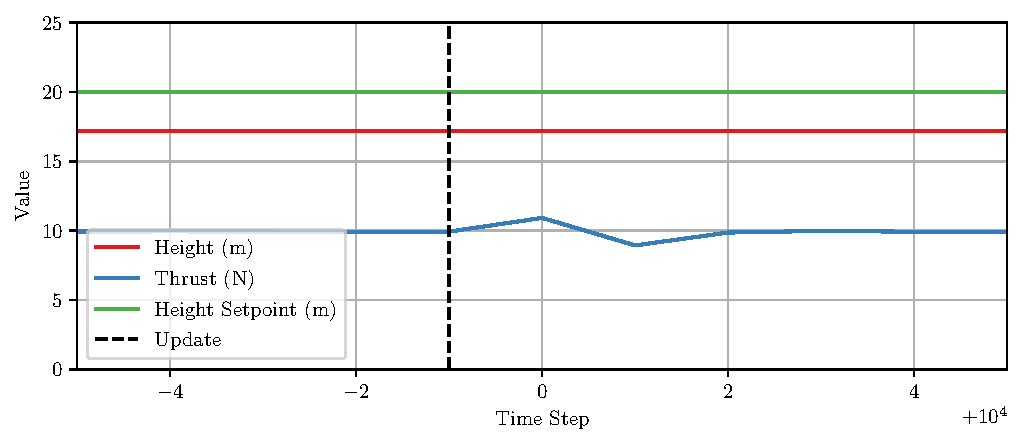
\includegraphics[width=\textwidth]{elafry-plant-data-zoom.pdf}
    \caption[Test plant control view (zoomed)]
    {Test plant control view (zoomed)}
    \label{fig:testPlantControlViewZoomed}
\end{figure}

\clearpage

\section{Future Research}

Blockchain

Edges, DSU also